% arara: xelatex: { shell: yes }
% arara: biber
% arara: nomencl
% arara: xelatex: { shell: yes }
% arara: xelatex: { shell: yes }
\documentclass[nolibertine, ngerman, algorithm, nomencl, minted]{ttlab-qualify}
% mögliche Optionen:
% - ngerman
% - english
% - minted
% - algorithm
% - nomencl
% - nolibertine
\usepackage{libertine}
\usepackage{biblatex}
%\usepackage{listings}
%\usepackage{natbib}
\usepackage{hyperref}
\hypersetup{
    colorlinks=true,      % Aktiviert farbige Links
    urlcolor=blue,        % URLs in Blau
    linkcolor=black,      % Interne Links (z.B. Abschnittsverweise) in Schwarz
    citecolor=black,      % Zitatverweise (Bibliographie) in Schwarz
    filecolor=black,      % Dateilinks in Schwarz
    menucolor=black       % Acrobat-Menülinks in Schwarz
}
\urlstyle{same}

\addbibresource{bib.bib}

\begin{document}

\titlehead{
  Kenan Khauto\\
  7592047\\
  B.Sc Informatik\\
  6\\
  kenan.khauto@stud.uni-frankfurt.de 
}
\subject{Seminararbeit Text Analytics}
\author{Kenan Khauto}
\title{Image Understanding}
\subtitle{Lernen visueller Konzepte beim Inferieren ohne finetuning}
\date{Abgabedatum: 11.03.2024}
\publishers{Goethe-Universität Frankfurt am Main\\Prof. Alexander Mehler}

\maketitle


\tableofcontents

\chapter{Einleitung}
Im Bereich der künstlichen Intelligenz und des maschinellen Lernens hat sich in den letzten Jahren eine bemerkenswerte Entwicklung 
vollzogen, insbesondere im Verständnis visueller Konzepte durch Modelle wie CLIP (Contrastive Language–Image Pretraining). 
Diese Modelle haben das traditionelle Paradigma, das umfangreiche Fine-Tuning und spezialisierte Datensätze erforderte, herausgefordert 
und bieten neue Wege, wie Maschinen Bilder und Texte in einem zusammenhängenden Rahmen verstehen können.


Die Kernfrage, die wir in diesem Seminar untersuchen, lautet: \glqq Wie können KI-Modelle wie CLIP visuelle Konzepte effektiv durch 
Inferenz verstehen und interpretieren, ohne dass ein umfangreiches Fine-Tuning erforderlich ist?\grqq Diese Frage berührt die Grundlagen 
der Art und Weise, wie maschinelle Lernmodelle trainiert und angewendet werden, insbesondere im Kontext der Integration von visuellen und 
textuellen Daten.


CLIP, ein Produkt von OpenAI, repräsentiert einen Durchbruch in der Art und Weise, wie Maschinen lernen, Bilder und Texte zu verbinden. 
Anstatt sich auf umfangreiche, spezialisierte Datensätze zu verlassen, nutzt CLIP ein breites Spektrum an Internetdaten und lernt, 
visuelle Konzepte direkt aus einer Vielzahl von Bildern und den dazugehörigen Beschreibungen zu extrahieren. Dieser Ansatz ermöglicht 
es dem Modell, eine breite Palette von visuellen Konzepten zu verstehen, ohne für jedes neue Konzept speziell angepasst zu werden.


In diesem Seminar werden wir die Mechanismen hinter CLIP und ähnlichen Modellen erforschen. Wir werden untersuchen, wie diese Modelle 
trainiert werden, ihre Fähigkeit, visuelle Daten zu interpretieren, und die Herausforderungen, denen sie gegenüberstehen, wie zum Beispiel 
die Behandlung von Verzerrungen und die Generalisierbarkeit ihrer Erkenntnisse. Darüber hinaus werden wir diskutieren, wie diese Technologien 
in verschiedenen Anwendungsfeldern eingesetzt werden könnten, von der automatisierten Bildbeschreibung bis hin zur Verbesserung 
der Mensch-Maschine-Interaktion.

\chapter{Hauptteil}
\section{Theoretischer Hintergrund}
Dieser Abschnitt stellt die theoretischen Grundlagen vor, die für das Verständnis der Funktionsweise von KI-Modellen wie CLIP (Contrastive Language–Image Pretraining) essentiell sind. Hier werden die Kernelemente des maschinellen Lernens, die Besonderheiten des Deep Learning und die Bedeutung des kontrastiven Lernens für die Verarbeitung von Bild- und Textdaten erörtert.

\subsection{Grundlagen des maschinellen Lernens}

Maschinelles Lernen ist ein Teilgebiet der künstlichen Intelligenz, das sich mit der Entwicklung von Algorithmen beschäftigt, die Computern das Lernen aus Daten ermöglichen. Die Hauptzielsetzung des maschinellen Lernens ist es, Muster in Daten zu erkennen und auf Basis dieser Muster Vorhersagen oder Entscheidungen zu treffen.

\textbf{Überwachtes vs. unüberwachtes Lernen:} Überwachtes Lernen bezieht sich auf Lernprozesse, bei denen das Modell anhand von Beispieldaten und bekannten Ausgabewerten trainiert wird. Unüberwachtes Lernen hingegen befasst sich mit dem Finden von Mustern oder Strukturen in Daten, ohne vorherige Kenntnis der Ausgabewerte.

\textbf{Verstärkendes Lernen:} Eine weitere wichtige Lernmethode ist das verstärkende Lernen, bei dem ein Modell durch Belohnungen lernt, bestimmte Aktionen in einer Umgebung auszuführen, um ein bestimmtes Ziel zu erreichen.

\subsection{Deep Learning und neuronale Netzwerke}

Deep Learning, eine Unterklasse des maschinellen Lernens, basiert auf künstlichen neuronalen Netzwerken mit vielen Schichten (sogenannten \glqq tiefen\grqq Netzwerken). Diese Netzwerke sind in der Lage, komplexe Muster in großen Datenmengen zu erkennen.

\begin{figure}[h]
	\centering
	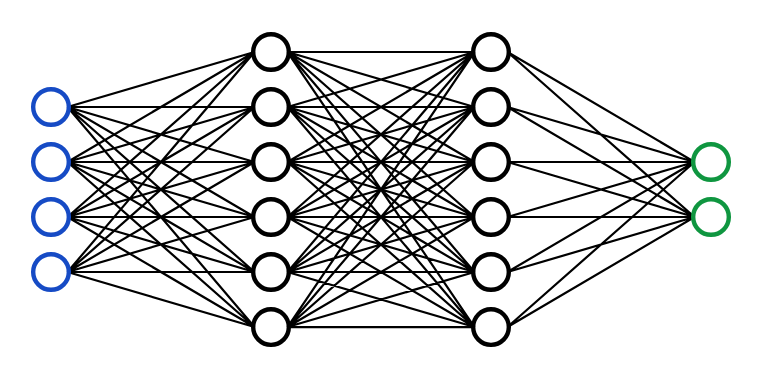
\includegraphics[scale=0.4]{static/FCnetwork.png}
	\caption{A simple fully connected neural network, see \url{https://victorzhou.com/series/neural-networks-from-scratch/}}
	\label{fig:2.1}
\end{figure}

\textbf{Convolutional Neural Networks (CNNs):} Speziell für die Bildverarbeitung (wie in \cite{oshea2015introduction} gezeigt wurde) sind CNNs von entscheidender Bedeutung. Sie sind darauf ausgelegt, hierarchische Muster in Bildern zu erkennen, was sie ideal für Aufgaben wie Bildklassifikation und Objekterkennung macht.
\begin{figure}[h]
	\centering
	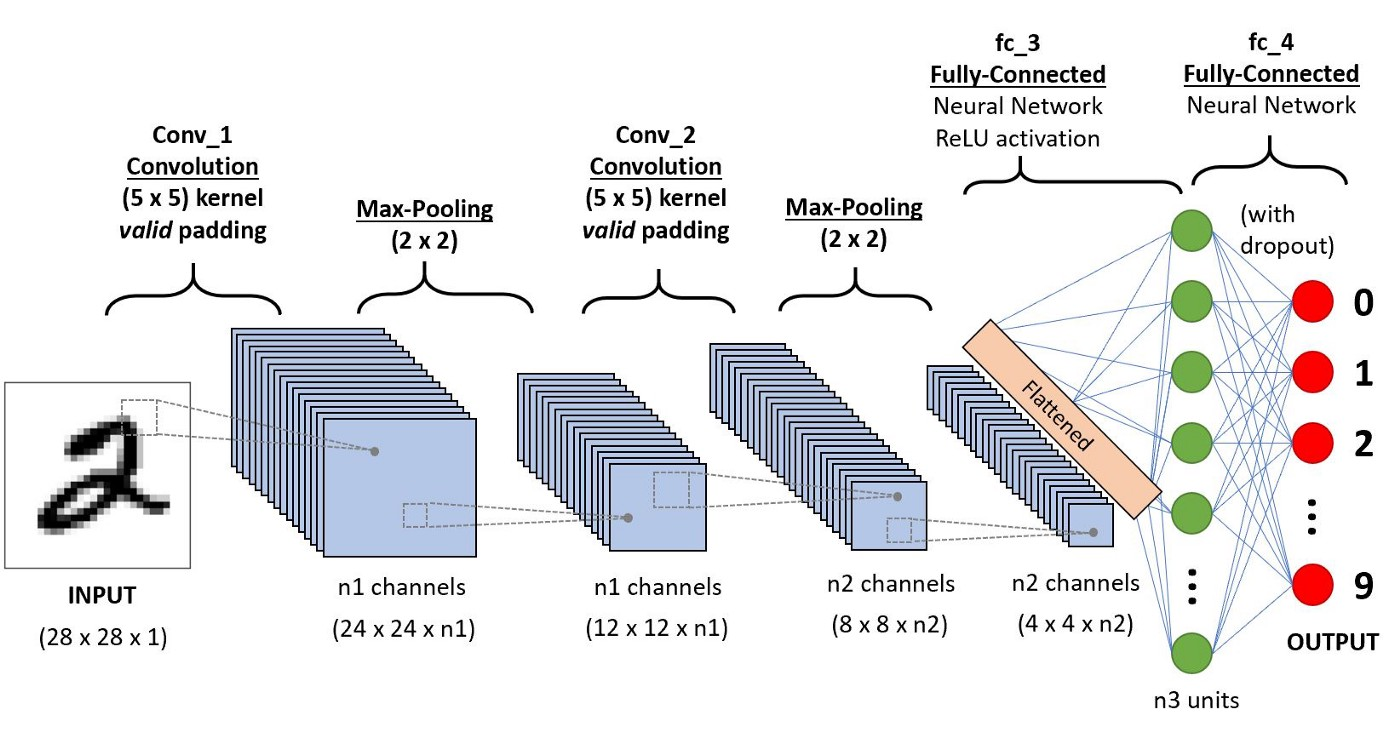
\includegraphics[scale=0.2]{static/cnn.jpeg}
	\caption{Convolutional neural network (CNN), see \url{https://paperswithcode.com/methods/category/convolutional-neural-networks}}
	\label{fig:2.2}
\end{figure}

\textbf{Transformer-Modelle:} Ursprünglich in der Verarbeitung natürlicher Sprache eingesetzt, haben Transformer-Modelle aufgrund ihrer Fähigkeit, langfristige Abhängigkeiten in Daten zu erkennen, zunehmend Anwendung in anderen Bereichen, einschließlich der Bildverarbeitung, gefunden.
\begin{figure}[h]
	\centering
	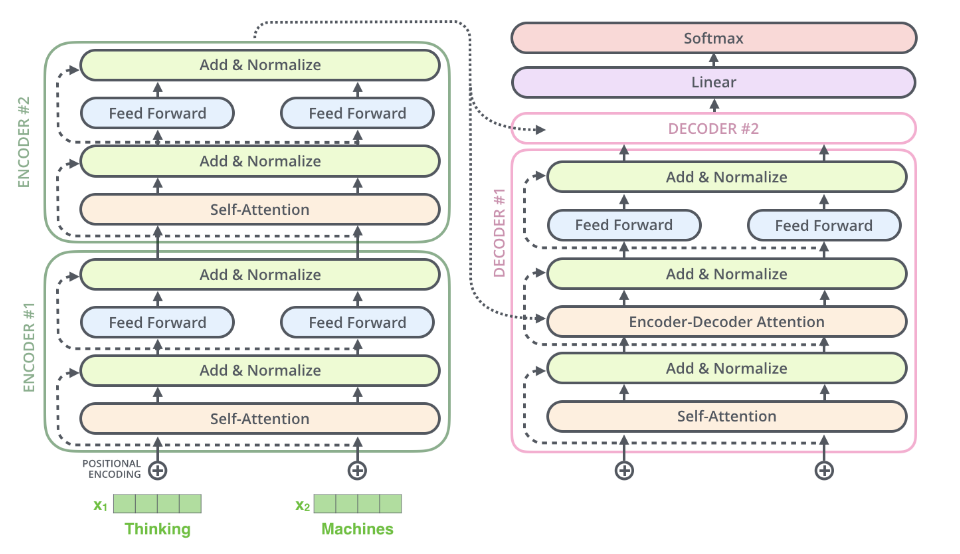
\includegraphics[scale=0.5]{static/transformer.png}
	\caption{Transformer with two encoders, 2 decoders and a fully connected layer for prediction, see \url{http://jalammar.github.io/illustrated-transformer/}}
	\label{fig:2.3}
\end{figure}

\subsection{Kontrastives Lernen und CLIP}
Kontrastives Lernen ist eine Technik, die darauf abzielt, ähnliche Datenpunkte näher zusammenzubringen und unähnliche weiter voneinander zu entfernen. CLIP verwendet kontrastives Lernen, um die Beziehungen zwischen Bildern und Text zu verstehen.

\textbf{Funktionsweise von CLIP:} CLIP wird mit einer Vielzahl von Bildern und den dazugehörigen Textbeschreibungen trainiert. Das Modell lernt, die Verbindungen zwischen Bildern und Texten zu verstehen, was es ihm ermöglicht, eine breite Palette von Bildinhalten effektiv zu interpretieren.

\textbf{Vorteile gegenüber traditionellen Ansätzen:} Im Gegensatz zu traditionellen Bilderkennungsmodellen, die oft umfangreiches Fine-Tuning für spezifische Aufgaben benötigen, kann CLIP vielfältige visuelle Konzepte anhand seiner Trainingsdaten erkennen und interpretieren, was eine größere Flexibilität und Anpassungsfähigkeit bedeutet.
\section{Analyse von CLIP}
CLIP \parencite{radford2021learning} ist ein neuronales Netzwerk, das anhand einer Vielzahl von Bildern und den zugehörigen Textbeschreibungen trainiert wurde. Dieses Training ermöglicht es ihm, sowohl visuelle als auch textuelle Eingaben zu verstehen und zu interpretieren. Im Gegensatz zu traditionellen Modellen, die eine aufgabenspezifische Feinabstimmung erfordern, ist CLIP für eine breite Palette visueller Aufgaben direkt einsetzbar.

\subsection{Architektur}
Das Modell besteht aus zwei Hauptkomponenten: einem Text-Encoder und einem Bild-Encoder. Der Text-Encoder verarbeitet textuelle Eingaben, während der Bild-Encoder sich um visuelle Eingaben kümmert. Beide Encoder wandeln ihre jeweiligen Eingaben in einen gemeinsamen Einbettungsraum um, was dem Modell ermöglicht, die beiden unterschiedlichen Datentypen direkt zu vergleichen und zu verknüpfen.
\begin{figure}[h]
	\centering
	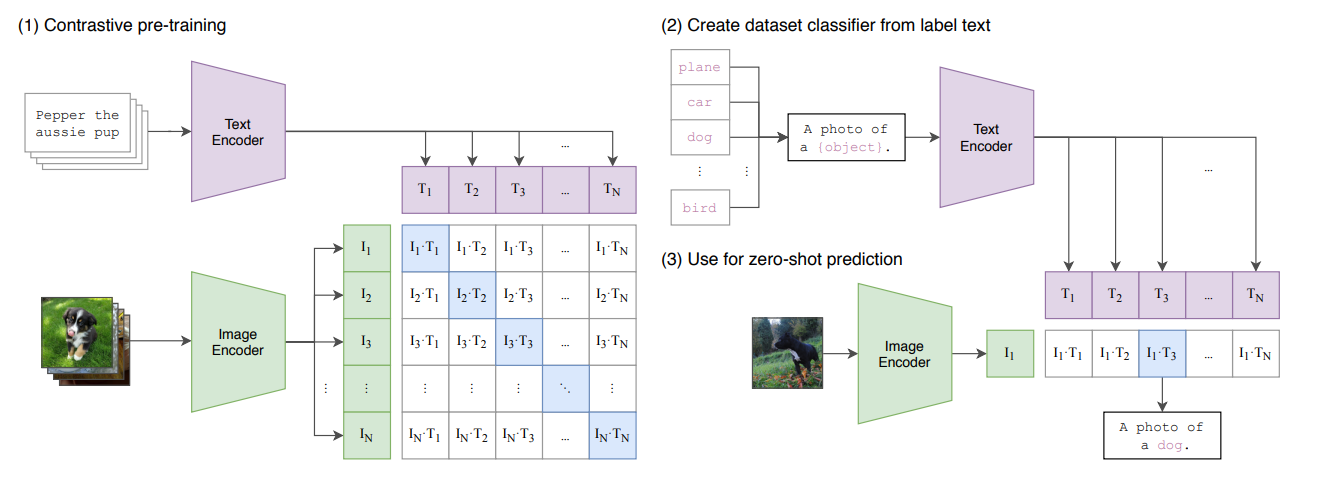
\includegraphics[scale=0.4]{static/CLIP.png}
	\caption{CLIP, Bild von \textcite[2]{radford2021learning}}
	\label{fig:2.4}
\end{figure}
\subsubsection{Text-Encoder}
Der Text-Encoder in CLIP basiert auf einer Transformer-Architektur. 
Jedes Wort im Text wird in eine Vektordarstellung umgewandelt. 
Der Transformer verwendet Selbst-Attention, um die Bedeutung jedes Wortes 
im Kontext des gesamten Textes zu verstehen. Ziel des Text-Encoders ist es, 
eine Darstellung des Textes zu erzeugen, die dessen semantischen Inhalt in Bezug auf mögliche Bildinhalte widerspiegelt.

Transformer-Modelle, eingeführt in dem Papier \glqq Attention is All You Need\grqq 
von \textcite{vaswani2017attention}, stellen einen Paradigmenwechsel in der 
Verarbeitung von Sequenzen dar, indem sie auf rekurrente Schichten verzichten 
und sich vollständig auf Mechanismen der Selbst-Attention und Positional-Encodings 
verlassen, um Sequenz-zu-Sequenz-Aufgaben zu bewältigen.

Die Selbst-Attention ist das Herzstück des Transformer-Modells. Sie ermöglicht es dem Modell, 
Abhängigkeiten zwischen allen Worten in einem Satz unabhängig von ihrer Entfernung zu lernen. 
Die Berechnung der Selbst-Attention erfolgt wie folgt:

\begin{figure}[h]
	\centering
	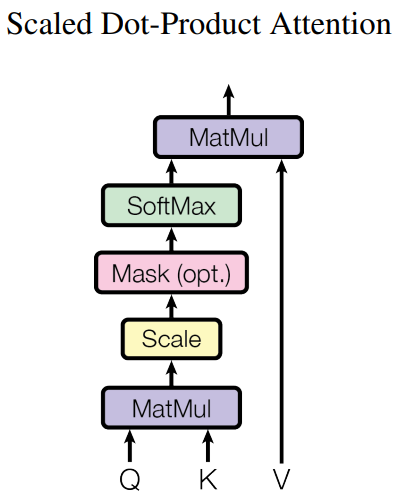
\includegraphics[scale=0.4]{static/attention.png}
	\caption{Scaled Dot-Product Attention, Bild von \parencite[4]{vaswani2017attention}}
	\label{fig:2.5}
\end{figure}

Gegeben sei eine Eingabesequenz $X$, bestehend aus $n$ Vektoren $x_1, x_2, \ldots, x_n$, 
wobei jedes $x_i \in \mathbb{R}^d$ ein Wortvektor ist. Zuerst werden drei Matrizen $Q$ (Query), 
$K$ (Key) und $V$ (Value) durch Multiplikation von $X$ mit den Gewichtsmatrizen $W^Q$, $W^K$ und $W^V$ berechnet:

\begin{align*}
	Q = XW^Q, \quad
	K = XW^K, \quad
	V = XW^V
\end{align*}
	
Anschließend wird die Attention-Matrix $A$ wie folgt berechnet:
	
\begin{align*}
	A = \text{softmax}\left(\frac{QK^T}{\sqrt{d_k}}\right)V
\end{align*}
	
Hierbei ist $d_k$ die Dimension der Key-Vektoren, und die Division durch $\sqrt{d_k}$ dient der Skalierung.

Da Transformer-Modelle keine rekurrente Struktur aufweisen, benötigen sie eine andere Methode, um Informationen über 
die Position von Wörtern in der Sequenz zu integrieren. Dies geschieht durch Positional Encoding, welches zu jedem Eingabevektor 
hinzugefügt wird:

\begin{align*}
	PE_{(pos, 2i)} = \sin\left(pos / 10000^{2i/d_{\text{model}}}\right) \\
	PE_{(pos, 2i+1)} = \cos\left(pos / 10000^{2i/d_{\text{model}}}\right)
\end{align*}

wobei $pos$ die Position und $i$ die Dimension ist. $d_{\text{model}}$ ist die Dimension der Wortvektoren.

\subsubsection{Bild-Encoder}
Der Bild-Encoder in CLIP ist nicht ausschließlich auf Convolutional Neural Networks (CNNs) beschränkt, sondern kann auch Vision Transformers (ViTs) umfassen. Die Wahl des spezifischen Netzwerktyps hängt von der gewünschten Leistung und den Eigenschaften der Aufgabe ab:
\begin{itemize}
    \item \textbf{CNN-basierte Encoder}: Traditionelle CNN-Architekturen (\textcite{lecun2015deep}, \textcite{krizhevsky2012imagenet}) 
	sind effektiv in der Erkennung lokaler Muster und Texturen in Bildern. Sie wandeln das Bild in eine Serie von 
	Vektorrepräsentationen um, die die visuellen Inhalte des Bildes kodieren.
    Convolutional Neural Networks (CNNs) sind eine Klasse von tiefen neuronalen Netzwerken, 
	die besonders effektiv in der Verarbeitung von Daten mit einer bekannten, grid-ähnlichen 
	Topologie sind, wie z.B. Bilder (2D-Grid von Pixeln). CNNs nutzen spezialisierte Schichten, 
	wie Faltungsschichten (Convolutional Layers), Pooling-Schichten und Fully-Connected (Dense) Layers, 
	um Merkmale aus den Daten zu extrahieren und zu lernen.

	Die Faltungsschicht ist das Kernstück eines CNN. Sie führt eine Faltungsoperation durch, 
	bei der ein Satz von lernbaren Filtern (oder Kernen) über das Eingabebild oder die Feature-Maps 
	gleitet, um neue Feature-Maps zu erzeugen. Für einen Filter \(F\) der Größe \(k \times k\) und 
	eine Eingabematrix \(X\) wird die Faltungsoperation wie folgt definiert:
	\begin{equation*}
		(S * F)_{i,j} = \sum_{m=0}^{k-1} \sum_{n=0}^{k-1} S_{i+m, j+n} \cdot F_{m,n}
	\end{equation*}
	wobei \((S * F)_{i,j}\) das Element der Ausgabe-Feature-Map an der Position \((i, j)\) ist.
	
	Die Pooling-Schicht dient dazu, die räumliche Größe der Feature-Maps zu reduzieren, 
	wodurch die Anzahl der Parameter und der Rechenaufwand im Netz verringert wird und 
	gleichzeitig die räumlichen Hierarchien der Merkmale erhalten bleiben. Die am häufigsten 
	verwendete Pooling-Operation ist das Max-Pooling, das aus einem Bereich von Werten den maximalen Wert auswählt.

	Nachdem mehrere Faltungs- und Pooling-Schichten angewendet wurden, folgen Fully-Connected Schichten, 
	die ähnlich wie in traditionellen neuronalen Netzwerken arbeiten. Diese Schichten erhalten eine flache 
	Liste von Features und führen klassische neuronale Netzoperationen durch, um die finale Klassifikation 
	oder Vorhersage zu berechnen.

	\item \textbf{Vision Transformers}: ViTs nähern sich der Bildverarbeitung auf eine andere Weise an, indem sie das Bild in eine Sequenz von Patches zerlegen und diese Patches ähnlich wie Wörter in einem Satz behandeln. Dies ermöglicht es ViTs, sowohl lokale als auch globale Kontextinformationen aus dem Bild zu erfassen.
\end{itemize}
Der Hauptzweck des Bild-Encoders, unabhängig von der gewählten Architektur, besteht darin, 
eine Darstellung des Bildes zu erzeugen, die in demselben Vektorraum wie der Text-Encoder liegt, 
um eine direkte Vergleichbarkeit und Verknüpfung von Text und Bild zu ermöglichen.

Für Leser, die sich tiefergehend mit der Theorie und Anwendung von Transformern beschäftigen möchten, 
empfehle ich die grundlegenden Papers \textcite{vaswani2017attention} und \textcite{dosovitskiy2020image}.
Diese zwei Werke bieten eine umfassende Einführung in das Konzept der Transformer und ViTs und legt 
den Grundstein für viele moderne Ansätze in der Verarbeitung natürlicher Sprache und Bilderkennung.

\subsection{Integration und gemeinsamer Einbettungsraum}
Die zentrale Innovation von CLIP besteht darin, dass beide Encoder - der Text- und der Bild-Encoder - darauf trainiert sind, ihre Ausgaben in einem gemeinsamen Einbettungsraum zu repräsentieren. Dies ermöglicht es dem Modell, die Beziehung zwischen Texten und Bildern effektiv zu verstehen und auf dieser Basis präzise Entscheidungen zu treffen.

\begin{itemize}
	\item \textbf{\textit{Vektorraumbildung: }} CLIP lernt, Bilder und Texte in einen hochdimensionalen Vektorraum zu transformieren. Dabei werden Bild- und Textrepräsentationen so angepasst, dass korrespondierende Paare nahe beieinander liegen.
	\item \textbf{\textit{Kontrastives Lernen: }}Das Modell verwendet einen kontrastiven Lernansatz, um die Distanz zwischen übereinstimmenden Bild-Text-Paaren zu minimieren und die Distanz zwischen nicht übereinstimmenden Paaren zu maximieren. Dieses Training fördert eine effektive Abbildung beider Modalitäten in den gemeinsamen Raum.
\end{itemize}

\subsection{Kontrastives Lernen im Detail}
Der kontrastive Lernansatz von CLIP basiert darauf, dass das Modell
lernt, korrespondierende Text-Bild-Paare miteinander zu verknüpfen,
während es gleichzeitig nicht passende Paare unterscheidet. Dieser
Ansatz erlaubt es dem Modell, eine umfassende und nuancierte Sicht
auf die Beziehungen zwischen Texten und Bildern zu entwickeln, was für die 
Zero-Shot-Lernfähigkeiten von CLIP entscheidend ist \parencite[5]{radford2021learning}.


\subsubsection{Vektoreinbettungen}
Sei \( \textbf{I} \) ein Bild und \( \textbf{T} \) ein Text, dann werden die Einbettungen durch die Encoder-Funktionen wie folgt generiert:
\begin{align*}
\text{Bild-Einbettung:} \quad & \textbf{v}_I = f_{\text{Bild}}(\textbf{I}) \\
\text{Text-Einbettung:} \quad & \textbf{v}_T = f_{\text{Text}}(\textbf{T})
\end{align*}
wobei \( f_{\text{Bild}} \) und \( f_{\text{Text}} \) die Funktionen des Bild- bzw. Text-Encoders sind.

\subsubsection{Ähnlichkeitsberechnung}
Die Ähnlichkeit zwischen einem Bild- und einem Textvektor wird durch das Skalarprodukt ihrer normalisierten Vektoren berechnet:
\begin{align*}
\text{sim}(\textbf{I}, \textbf{T}) = \frac{\textbf{v}_I \cdot \textbf{v}_T}{\| \textbf{v}_I \| \, \| \textbf{v}_T \|}
\end{align*}

Das kann man in \ref{fig:2.4} sehen.
\subsubsection{Training und kontrastiver Verlust}
Das Training von CLIP erfolgt durch Minimierung des kontrastiven Verlustes. Für ein Batch von \( N \) Bild-Text-Paaren wird der Verlust für ein Paar \( (T, I) \) berechnet als:
\begin{align*}
L_{T,I} = -\log \frac{\exp(\text{sim}(\textbf{v}_{I}, \textbf{v}_{T}) / \tau)}{\sum_{T´} \exp(\text{sim}(\textbf{v}_{I}, \textbf{v}_{T´}) / \tau)} - \log \frac{\exp(\text{sim}(\textbf{v}_{T}, \textbf{v}_{I}) / \tau)}{\sum_{I´} \exp(\text{sim}(\textbf{v}_{T}, \textbf{v}_{I´}) / \tau)} 
\end{align*}
Hierbei ist:
\begin{itemize}
 \item \( \tau \) ein Temperaturparameter ist, der die Schärfe der Wahrscheinlichkeitsverteilung beeinflusst,
 \item Die Summen laufen über alle Texte und Bilder jeweils
\end{itemize}

Diese Formel zielt darauf ab, die Wahrscheinlichkeit zu maximieren, dass das korrekte Bild-Text-Paar unter 
Berücksichtigung aller anderen Paare im Batch als das ähnlichste Paar ausgewählt wird. Der Logarithmus im 
Zähler bewirkt, dass das korrekte Paar einen hohen Beitrag zum Gesamtverlust leistet, wenn es nicht als ähnlichstes 
Paar identifiziert wird. Im Nenner summiert sich der Beitrag aller Paare im Batch, was die Unterscheidung zwischen 
korrekten und inkorrekten Paaren fördert.

\subsubsection{Gesamtverlust}
Für ein Batch mit $N$ Bild-Text Paare, wird die Gesamtverlust mit:
\begin{align*}
	L_{total} = \frac{1}{N} \sum_{i=1}^{N} L(I_i, T_i)
\end{align*}
berechnet.

Die symmetrische Natur der Loss-Funktion (symmetric Cross Entropy Loss) stellt sicher, 
dass die Bild-zu-Text- und Text-zu-Bild Vorhersagen während des Trainings gleichmäßig betont werden.

\subsection{Zero-Shot Learning in CLIP}
\subsubsection{Konzept}
Zero-shot bedeutet die Anwendung eines Modells ohne die Notwendigkeit des Feintunings. 
Das bedeutet, dass wir ein Modell nehmen und es verwenden, um Bilder in einem 
bestimmten Bereich zu detektieren, und dann zu einem vollständig anderen Bereich wechseln, 
ohne dass das Modell auch nur ein einziges Trainingsbeispiel aus dem neuen Bereich gesehen hat.

Zero-Shot Learning bezieht sich auf die Fähigkeit des Modells,
Aufgaben zu verstehen und durchzuführen, für die es nicht 
explizit trainiert wurde. Im Kontext von CLIP bedeutet dies, 
Bilder und Konzepte zu erkennen und zu interpretieren, 
die es während des Trainings nie gesehen hat.

\subsubsection{Mechanismus}
Dies wird durch das generalisierte Verständnis des Modells von Bildern und Texten 
erreicht. Durch das Training mit einem vielfältigen Datensatz lernt CLIP eine breite 
Palette von visuellen Stilen, Objekten und Konzepten, was ihm eine gute Generalisierung 
auf neue, ungesehene Aufgaben ermöglicht.

\subsubsection{Beispiel Code für Image Classification}
Diese Eigenschaft macht CLIP außerordentlich vielseitig. Es kann für verschiedene 
Aufgaben wie Objekterkennung, Inhaltsmoderation und sogar kreative Anwendungen wie 
das Generieren von Bildern aus Textbeschreibungen verwendet werden.

Im Folgenden werden ich einen Beispiel Code von \textcite{pinecone2023zeroshot} zeigen, wie man mit CLIP Image Classification machen kann.
Dafür brauchen wir das Modell von OpenAI. Und dann noch den CLIP-Processor.
Der Processor ist dafür zuständig, die Labels und Images in eine passende Form für CLIP umzuwandeln.

\begin{minted}[frame=lines, framesep=2mm, baselinestretch=1.2, fontsize=\footnotesize]{python}

from transformers import CLIPProcessor, CLIPModel
model_id = "openai/clip-vit-base-patch32"
processor = CLIPProcessor.from_pretrained(model_id)
model = CLIPModel.from_pretrained(model_id)

image = read_image(image_name="2.jpg")
image = np.expand_dims(image, axis=0)

labels = ["A photo of a piano", 
"Someone playing the piano", 
"A photo of a guitar", 
"A photo of a piano in a white background",
"A very big dog eating hotdogs", 
"A fluffy cat", 
"A photo of the earth from the dark space"]

labels = processor(
text=labels,
images=None,
padding=True,
return_tensors="pt"
).to(device)

text_emb = model.get_text_features(**labels)
text_emb = text_emb.detach().cpu().numpy()
text_emb = text_emb / np.linalg.norm(text_emb, axis=0)

image = processor(
text=None,
images=image,
return_tensors="pt"
)["pixel_values"].to(device)

image_emb = model.get_image_features(image)
image_emb = image_emb.detach().cpu().numpy()

similarities = np.dot(image_emb, text_emb.T)

index = np.argmax(similarities, axis=1).item()

result = labesl[index]
\end{minted}

Der komplette Code findet man auf \url{https://github.com/KenanKhauto/zero-shot-learning}.
Die Labels habe ich selber manuell erstellt.
Und das Bild, was ich als Eingabe benutzt habe, ist ein Klavier mit einem weißen Hintergrund. Und die Ausgabe des Models ist auch diese Beschreibung.
Das zeigt vorallem, dass das Model nicht nur Objekte klassifiziert, sondern auch das komplette Bild versteht.
\subsection{Vergleichsanalyse}

\subsubsection{Traditionelle Vision-Modelle}
Frühere Modelle in der Computer Vision waren in der Regel aufgabenspezifisch (z.B. Modelle zur Objekterkennung, Bildsegmentierung) und erforderten umfangreiche Feinabstimmungen mit beschrifteten Daten für jede Aufgabe.
\begin{figure}[h]
	\centering
	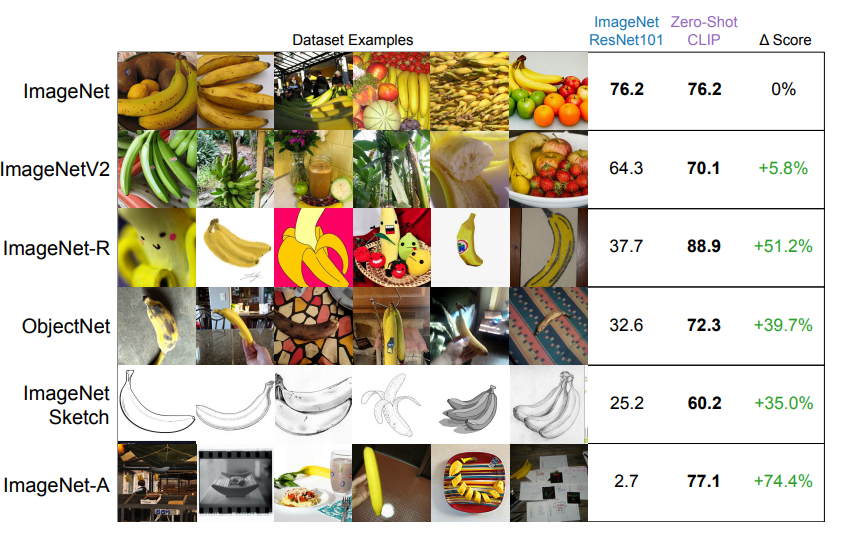
\includegraphics[scale=0.5]{static/resnet_vs_clip.png}
	\caption{Resnet-101 fine-tuned on ImageNet vs. zero-shot CLIP, Bild von \textcite[15]{radford2021learning}}
	\label{fig:2.7}
\end{figure}

In diesem Vergleich (\ref{fig:2.7}) können wir sehen, dass trotz des Trainings von ResNet-101 für ImageNet seine Performanz bei 
ähnlichen Datensätzen viel schlechter ist als die von CLIP bei denselben Aufgaben. CLIP übertrifft ein SotA-Modell, 
das für ImageNet trainiert wurde, bei leicht modifizierten ImageNet-Aufgaben.

Wenn ein ResNet-Modell auf andere Domänen angewendet wird, ist ein Standardansatz die Verwendung einer „linear probe“. 
Dabei werden die gelernten Merkmale von ResNet (aus den letzten paar Layers) in einen linearen Classifier eingespeist, 
der dann für einen spezifischen Datensatz fine-tuned wird. Dies würde man als Few- bis Many-Shot-Learning bezeichnen.

\begin{figure}[h!]
	\centering
	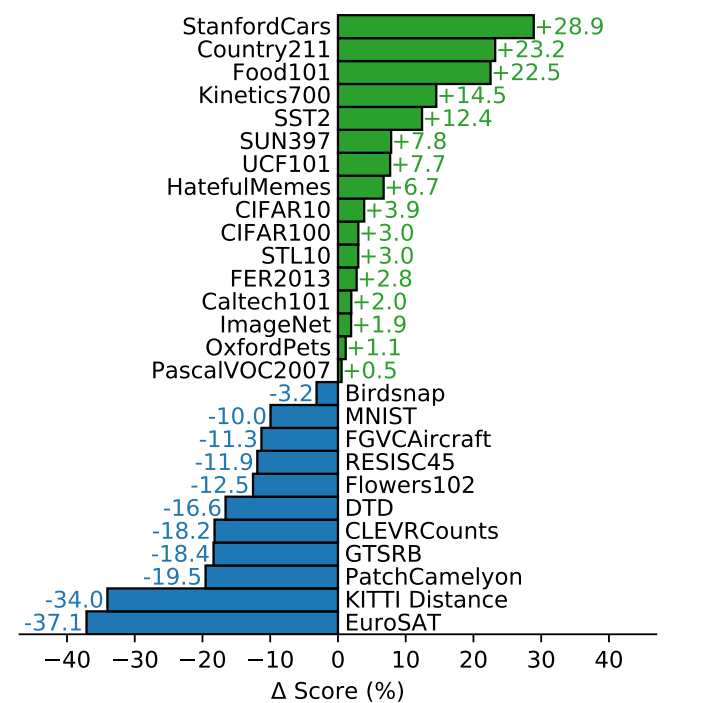
\includegraphics[scale=0.4]{static/clip_vs_resnet50.png}
	\caption{Linear Probe on ResNet50 vs. zero-shot CLIP, Figur von \textcite[8]{radford2021learning}}
	\label{fig:2.8}
\end{figure}


In \ref{fig:2.8} \parencite[vgl.][]{radford2021learning} wurde das linear probe von ResNet-50 mit dem Zero-Shot-CLIP verglichen. 
In einem Szenario übertrifft Zero-Shot-CLIP das linear probe bei vielen Aufgaben.


\section{Anwendungen}
\label{sec:Anwendung}
\subsection{Zero-Shot-Classifier auf CIFAR10}
Im Folgenden präsentiere ich eine Tabelle, die die Ergebnisse verschiedener Prompts und ihre Genauigkeit bei der 
Klassifizierung von Bildern des CIFAR-10-Datensatzes zusammenfasst. Die Ergebnisse verdeutlichen, wie die Wahl des 
Prompts die Leistungsfähigkeit des Zero-Shot-Klassifikators beeinflusst.

\begin{table}[h!]
	\centering
	\begin{tabular}{lll}
	  \toprule
	  Prompt & Accuracy & Comment \\
	  \midrule
	  'This is a \{\}' & 0.696 & not so good \\
	  'A \{\}' & 0.672 & Poor result \\
	  '\{\}' & 0.708 & Could be better... \\
	  'This image contains \{\}' & 71.5 & Improvement, but not significantly better \\
	  'There is \{\}' & 71.5 & Improvement, but not significantly better \\
	  'a photo of a \{\}' & 0.716 & better \\
	  'you can see a \{\}' & 0.716 & better \\
	  'A \{\} is in the picture' & 0.726 & better \\
	  'In this image you can see a \{\}' & 0.727 & Best result so far \\
	  'You can see a \{\} in this image' & 0.727 & Best result so far \\
	  'An \{\} is waiting' & 0.733 & best \\
	  \bottomrule
	\end{tabular}
	\caption{Eigene Ergebnisse von Zero-Shot CLIP auf CIFAR10}
  \end{table}

\subsection{Bild- und Textsuche}
CLIP kann eine Brücke zwischen Bildern und Texten schlagen, indem es eine gemeinsame Darstellungsweise im 
gleichen Vektorraum ermöglicht. Wenn zum Beispiel ein Nutzer nach \glqq einem Strand bei Sonnenuntergang\grqq sucht, 
analysiert CLIP die Textanfrage und vergleicht sie mit den erlernten visuellen Repräsentationen von Bildern in 
seiner Datenbank, um die passenden Bilder zu finden. Umgekehrt kann bei der Eingabe eines Bildes CLIP ähnliche 
Textbeschreibungen oder Keywords liefern, die den Inhalt des Bildes beschreiben.

\subsection{Automatische Bildbeschriftung}
Die automatische Bildbeschriftung ist ein Prozess, bei dem einem Bild eine passende Textbeschreibung zugeordnet wird. 
CLIP kann diese Aufgabe durchführen, indem es die visuellen Elemente eines Bildes analysiert und diese Informationen 
dann verwendet, um eine genaue und relevante Beschreibung in natürlicher Sprache zu generieren. Dies ist besonders 
nützlich für die Barrierefreiheit, um sehbehinderten Nutzern Inhalte zugänglich zu machen, sowie für die automatische 
Generierung von Alt-Texten für Bilder im Web.

\subsection{Sentiment-Analysis in Bildern}
Die Sentiment-Analyse, traditionell auf Texte angewandt, kann mit CLIP auch auf Bilder übertragen werden. 
CLIP kann die Stimmung oder das Gefühl erkennen, das ein Bild vermittelt, indem es die visuellen Elemente 
und deren Assoziationen mit emotionalen Zuständen interpretiert. Dies könnte für Marken wertvoll sein, um zu 
verstehen, wie ihre Produkte in sozialen Medien wahrgenommen werden, oder in der psychologischen Forschung, 
um emotionale Reaktionen auf visuelle Stimuli zu untersuchen.


\subsection{Bildgeneration mit Text Prompts}
In diesem Abschnitt zeige ich Beispiele über Prompts und Antworten von ChatGPT4, die es ermöglichen, Bilder mithilfe von Text-Prompts zu generieren. Es wird 
mithilfe von DALLE generiert.\\
\textbf{Me:} Can you generate an Image of a futuristic city?\\
\textbf{ChatGPT4:} Here's an image of a futuristic cityscape, capturing the essence of a 
technologically advanced urban environment under a twilight sky. The city is a blend of 
ultra-modern architecture, sustainable living elements, and advanced transportation systems, 
designed to offer a glimpse into what urban life could look like in a future driven by technology and innovation.
\begin{figure}[h!]
	\centering
	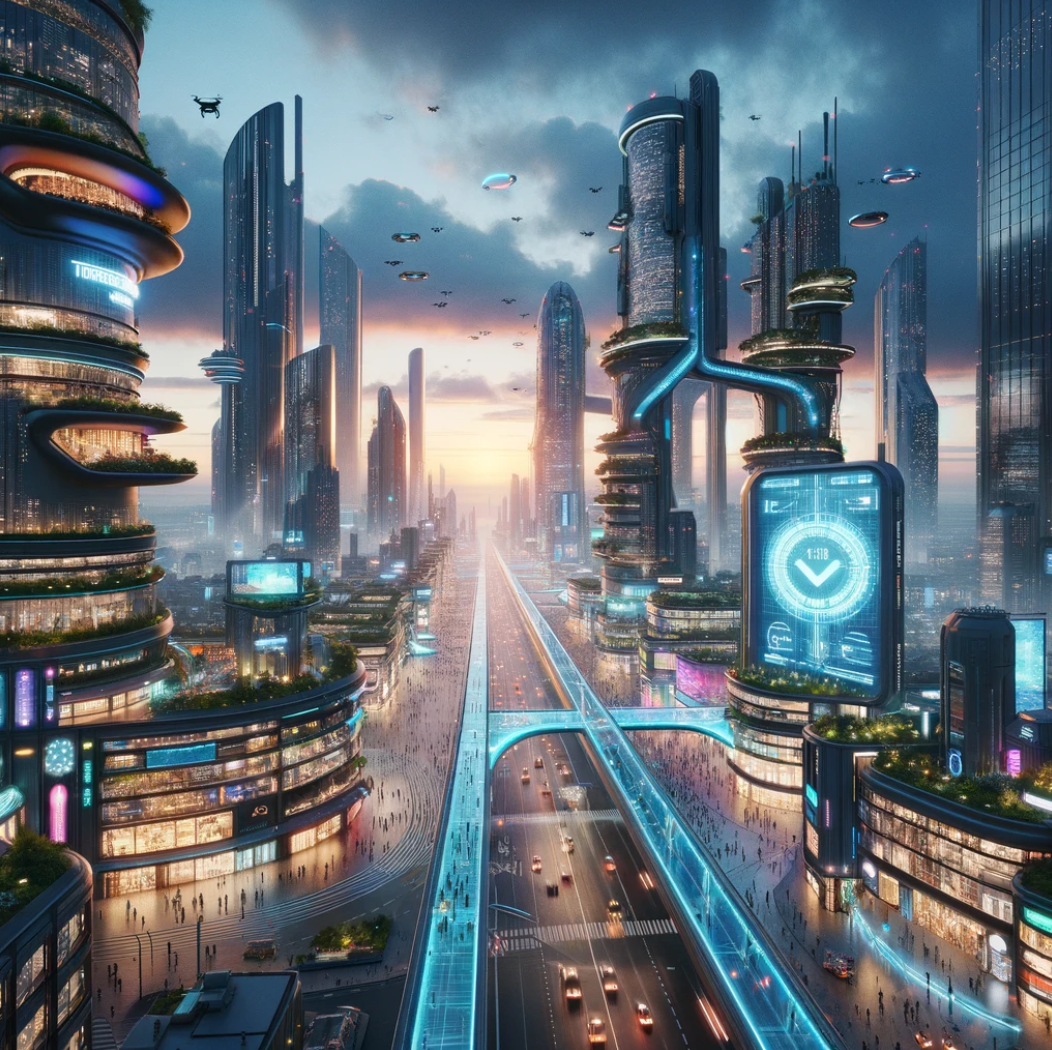
\includegraphics[scale=0.2]{static/fcity.png}
\end{figure}
\\
\textbf{Me:} Can you add a Baroque style to it ?\\
\textbf{ChatGPT4:} I've added a Baroque influence to the futuristic cityscape. This unique fusion brings together 
the elaborate and ornate architectural style of the 17th century with modern and sustainable elements, creating a 
vivid representation of how the past and future can intertwine in urban design.
\begin{figure}[h!]
	\centering
	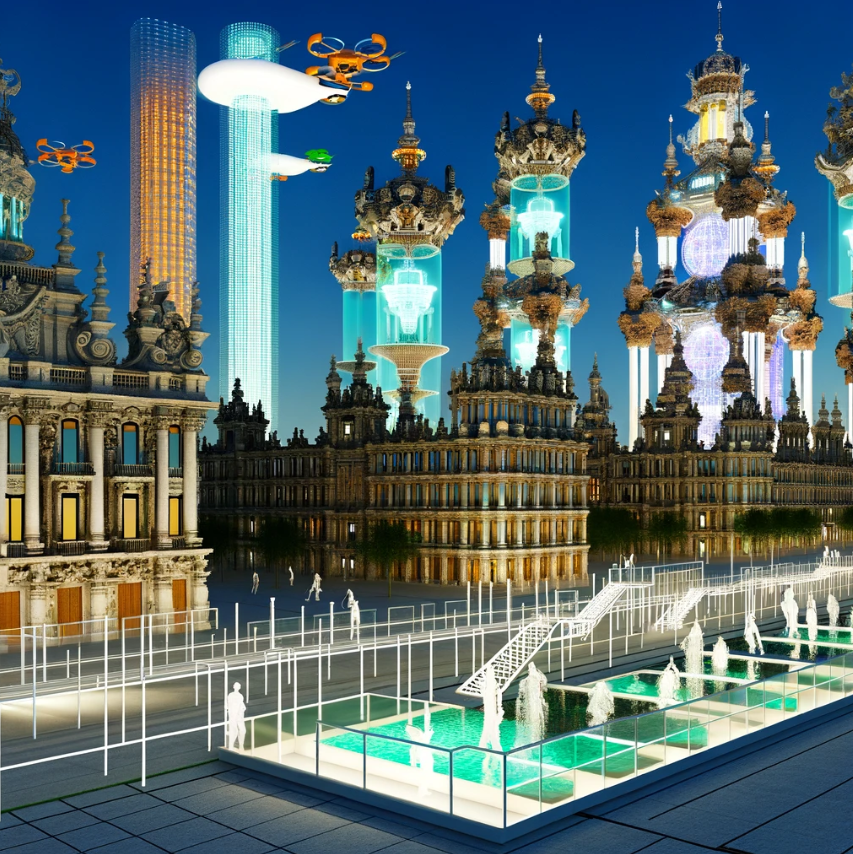
\includegraphics[scale=0.2]{static/fcity_barock.png}
\end{figure}



\section{Diskussion von Herausforderungen und Grenzen}
\subsection{Datensatz- und Verzerrungsprobleme}
Ein wesentliches Problem bei der Entwicklung von CLIP-ähnlichen Modellen ist die Qualität und Vielfalt der Daten, 
mit denen sie trainiert werden. Die Modelle lernen, indem sie Muster aus den Trainingsdaten extrahieren. Wenn die 
Daten verzerrt sind oder bestimmte Bevölkerungsgruppen nicht ausreichend repräsentieren, kann dies zu einem biased (verzerrten) 
Modellverhalten führen. Ein Beispiel für eine solche Verzerrung ist das Gender-Bias, bei dem das Modell dazu neigt, Berufe oder 
Aktivitäten stereotyp mit einem bestimmten Geschlecht zu verknüpfen.

\subsection{Generalisierbarkeit und Übertragbarkeit}
Obwohl CLIP erstaunliche Fähigkeiten bei Zero-Shot-Learning-Aufgaben zeigt, ist seine Fähigkeit, auf völlig neue Kontexte 
oder Domänen zu generalisieren, begrenzt. Die Übertragbarkeit von in einem Kontext gelernten Konzepten auf einen anderen ist 
eine fortlaufende Herausforderung in der KI. Das bedeutet, dass CLIP unter Umständen nicht effektiv funktioniert, wenn es mit 
Bildern oder Texten konfrontiert wird, die stark von seinem Trainingsset abweichen.

\subsection{Interpretierbarkeit und Erklärbarkeit}
Wie bei vielen tiefen Lernmodellen ist auch bei CLIP die Interpretierbarkeit der Entscheidungen eine Herausforderung. 
Es ist oft nicht transparent, welche Merkmale des Datenmaterials das Modell für seine Vorhersagen heranzieht, 
was insbesondere dann problematisch wird, wenn fehlerhafte oder unethische Entscheidungen getroffen werden.

\subsection{Rechen- und Umweltbedenken}
Die Entwicklung und das Training von großangelegten Modellen wie CLIP erfordern erhebliche Rechenressourcen, 
was sowohl ökonomische als auch ökologische Bedenken aufwirft. Die CO2-Fußabdrücke, die durch das Training solcher 
Modelle entstehen, sind beträchtlich und werfen Fragen nach der Nachhaltigkeit solcher Technologien auf.

\subsection{Ethische und soziale Auswirkungen}
CLIP und ähnliche Technologien stellen eine Reihe von ethischen Fragen, insbesondere in Bezug auf Privatsphäre und Überwachung. 
Die Fähigkeit, Bilder und Texte in großem Umfang zu analysieren, kann ohne angemessene Kontrollen und Richtlinien zum Missbrauch 
führen. Es muss ein Gleichgewicht zwischen der Nutzung solcher Technologien zur Verbesserung von Dienstleistungen und dem Schutz 
der Rechte der Individuen gefunden werden.

\subsection{Missbrauchspotential}
Die leistungsfähige Verknüpfung von Bildern und Texten kann auch für schädliche Zwecke genutzt werden, beispielsweise zur 
Erstellung überzeugender Deepfakes oder zur Verbreitung von Desinformation. Die Erkennung und Abwehr solcher Bedrohungen ist 
eine signifikante Herausforderung für die Entwickler von KI-Systemen und für die Gesellschaft als Ganzes.

\subsection{Grenzen der Zero-Shot-Kapazitäten}
Obwohl CLIP in der Lage ist, ohne spezifische Anpassungen eine Vielzahl von Aufgaben zu erledigen, gibt es Grenzen dessen, 
was es im Zero-Shot-Modus erreichen kann. Insbesondere bei komplexen oder nuancierten Aufgaben, die ein tiefes Verständnis 
des Kontextes erfordern, kann CLIP weniger effektiv sein.

Diese Herausforderungen zeigen, dass, während CLIP und ähnliche Modelle beeindruckende technologische Fortschritte darstellen, 
ihre Entwicklung und Anwendung wohlüberlegt und verantwortungsbewusst erfolgen muss. Forschung und Entwicklung in Richtung fairerer, 
transparenterer und umweltfreundlicherer KI-Modelle ist entscheidend, um das volle Potenzial dieser Technologien zu realisieren, 
ohne unerwünschte Nebenwirkungen zu riskieren.

\section{Zukünftige Richtungen und mögliche Verbesserungen}
\subsection{Erweiterte Datensätze und Fairness}
Eine Hauptpriorität für die Weiterentwicklung von CLIP-ähnlichen Modellen ist die Erstellung und Nutzung von umfangreichen und 
vielfältigen Datensätzen. Zukünftige Forschung wird sich darauf konzentrieren müssen, Bias in Datensätzen zu erkennen und zu verringern, 
um faire und unparteiische KI-Modelle zu schaffen. Dies umfasst nicht nur eine gleichmäßigere Repräsentation verschiedener demographischer 
Gruppen, sondern auch die Sicherstellung, dass die trainierten Modelle eine faire Behandlung für alle Nutzer gewährleisten.

\subsection{Verbesserte Generalisierung und Adaption}
Um die Generalisierbarkeit von CLIP zu erhöhen, könnten zukünftige Modelle mehrschichtige Ansätze verfolgen, die es ermöglichen, 
abstrakte Konzepte besser zu erfassen und auf neue Domänen zu übertragen. Fortschritte in Transfer-Learning und Domain-Adaption könnten 
die Flexibilität von CLIP in einer Vielzahl von Anwendungsfällen wesentlich erweitern.

\subsection{Erhöhte Transparenz und Erklärbarkeit}
Ein kontinuierliches Ziel ist es, die Entscheidungsfindung von CLIP transparenter und nachvollziehbarer zu gestalten. Forschung in den 
Bereichen erklärbares AI (XAI) könnte Wege aufzeigen, wie Modelle ihre Entscheidungen auf eine Art und Weise kommunizieren können, die für 
Menschen verständlich und nachprüfbar ist.

\subsection{Umweltfreundlichere KI}
Angesichts der Umweltbedenken, die mit dem Training großer KI-Modelle einhergehen, ist die Entwicklung energieeffizienterer Trainingsmethoden 
ein wichtiges Forschungsziel. Dies könnte durch verbesserte Hardware, optimierte Algorithmen oder durch die Verwendung von Methoden des sparsamen 
Lernens (Sparse Learning) erreicht werden.

\subsection{Ethische Richtlinien und Regulation}
Die Entwicklung von Richtlinien und regulatorischen Rahmenbedingungen wird eine Schlüsselrolle spielen, um sicherzustellen, dass die Vorteile 
von KI-Technologien maximiert und ihre Risiken minimiert werden. Dies schließt Maßnahmen zur Kontrolle von Missbrauch und zur Wahrung der Privatsphäre ein.

\subsection{Bekämpfung von Missbrauch}
Die Forschung muss sich ebenfalls auf die Erkennung und Prävention des Missbrauchs von KI-Modellen konzentrieren, wie z.B. die Erstellung von 
Deepfakes. Fortschritte in der Erkennung von Anomalien und der Authentifizierung von Inhalten können dazu beitragen, die Integrität von Informationen zu schützen.

\subsection{Fortschritt der Zero-Shot-Technologien}
Schließlich besteht ein stetiges Interesse daran, die Zero-Shot-Learning-Fähigkeiten von CLIP zu erweitern. Dies könnte die Erforschung neuer 
Architekturen, Trainingsmethoden und die Einbeziehung zusätzlicher Modalitäten wie Audio oder haptische Informationen umfassen.

Zusammenfassend lässt sich sagen, dass die Zukunft von CLIP und ähnlichen multimodalen KI-Systemen von der gleichzeitigen Entwicklung auf 
technologischer, sozialer und regulatorischer Ebene abhängt. Interdisziplinäre Ansätze, die technische Innovation mit ethischen Überlegungen 
und Umweltschutz verbinden, werden entscheidend sein, um das volle Potenzial dieser Technologien auszuschöpfen und gleichzeitig die Gesellschaft 
vor potenziellen Schäden zu schützen.

\printbibliography
\end{document}
